\section{Subspace Clustering}
The main idea of subspace clustering is to identify subspaces of a high dimensional space to allow better clustering than the original (full) space. This is opposed to e.g. PCA, which projects the original space onto a new subspace, which may can be hard to interpret for the user.

Two different subspace clustering approaches will be discussed. First, the grid-based approach will be discussed, after which the density-based approach will be discussed. Note that, only bottom-up approaches will be considered in this paper.

We will adopt the following notation: Let $\mathcal{A} = \{A_1, \dots, A_d\}$ be a set of domains, and $\mathcal{S} = A_1 \times A_2 \times \dots A_d$ a $d$-dimensional numerical space containing $n$ points $p_1, \dots, p_n$. Let $A_1, \dots, A_d$ be the dimensions (attributes) of $\mathcal{S}$.

\subsection{Grid-based approach}
The key idea of grid-based subspace clustering is to partition the $\mathcal{S}$ into axis-parallel grid structure starting in 1-dimensional space. The grids forms hyper-rectangular \textit{units} (cells) for which we find the number of points in each. Only the units that exceeds a certain threshold are retained, called \textit{dense units}. Next, adjacent dense units will be merged to form so called \textit{candidate dense units} (CDUs), which will be used to find clusters in higher dimensional subspaces. The goal is then to describe the clusters using a minimal description in the form of DNF (\textit{Disjunctive Normal Form}) expressions.

\subsubsection{CLIQUE}
CLIQUE is a bottom-up, grid-based subspace clustering algorithm that uses the monotonicity property as its clustering criterion, as described in Lemma \ref{lem:mono}:

\begin{lemma}\label{lem:mono}
    If a collection of points $S$ is a cluster in a $k$-dimensional subspace, then $S$ is also part of a cluster in any $(k-1)$-dimensional projection of this space.
\end{lemma}

The proof is provided in \cite{clique}.

The algorithm begins by partitioning the dataset $\mathcal{S}$ into equal-sized intervals of width $\varepsilon$ (input parameter), creating axis-parallel rectangular units. It then scans the dataset to identify 1-dimensional (1D) dense units by counting the number of points in each interval using a histogram, as shown in Figure \ref{fig:dense_cells_and_regions}. For example, with a grid size of $\varepsilon = 0.2$, three intervals in dimension $A_1$ exceed the density threshold $\tau$ (input parameter), while dimension $A_2$ reports four dense units. These dense units are known as \textit{candidate dense units} (CDUs).

The algorithm proceeds incrementally: it starts from 1D and moves to 2D, 3D, and so on, until no more CDUs can be generated. At each stage, the algorithm makes another pass over the dataset to determine which CDUs are dense in the higher dimensions, using the $(k-1)$-dimensional dense units identified in the previous stage. Specifically, CDUs in $k$ dimensions are formed by merging dense units in $(k-1)$ dimensions that share the first $(k-2)$ dimensions. This process continues until no further CDUs are generated.

To optimize performance, CLIQUE applies a pruning technique called \textit{coverage} (from \cite{clique}) to reduce computation time. This technique prunes subspaces with low coverage (i.e., those containing fewer points). However, this may risk eliminating subspaces that could potentially contain clusters.

Once all dense units are identified, CLIQUE defines clusters as maximal sets of connected dense units. For each $k$-dimensional subspace, the algorithm computes disjoint sets of connected dense units, where two units are connected if they share $k-1$ dimensions (a common face in the $k$-dimensional space) or if they are indirectly connected through other units. The algorithm then generates minimal cluster descriptions by covering each set of connected dense units with maximal regions and determining the minimal cover. For instance, in Figure \ref{fig:dense_cells_and_regions}, the minimal cover of the clusters is $A \cup B$, expressed as: $((0.2 \leq A_1 < 0.6) \land (0.4 \leq A_2 < 0.8)) \lor ((0.4 \leq A_1 < 0.8) \land (0.2 \leq A_2 < 0.6))$.
\begin{figure}[H]
    \vspace*{-0.5cm}
    \centering
    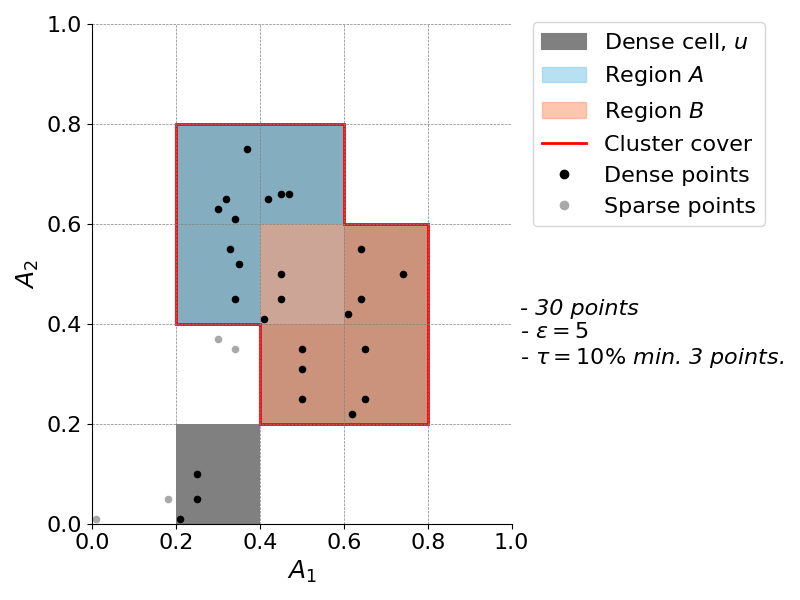
\includegraphics[width=0.35\textwidth]{figures/dense_cells_and_regions.png}
    \caption{Illustration of a dense unit $u$ and two overlapping dense regions $A$ and $B$.}
    \label{fig:dense_cells_and_regions}
    \vspace*{-0.5cm}
\end{figure}

\subsection{MAFIA}
MAFIA is an extension to CLIQUE where the grid sizes are adaptive meaning that the grid sizes are not fixed but are automatically determined by an algorithm. The idea is to cosim-2012ncentrate the portions of the data space, as having more points a more likely to be part of a cluster region enabling minimal length DNF expressions. The overall intention is not to rely on the input parameters CLIQUE uses do not use on the pruning technique as noted in cite{clique}, this could result in lost information. The algorithm is described in more detail in Section \ref{sec:mafia}.
\begin{figure}[H]
    \vspace*{-0.5cm}
    \centering
    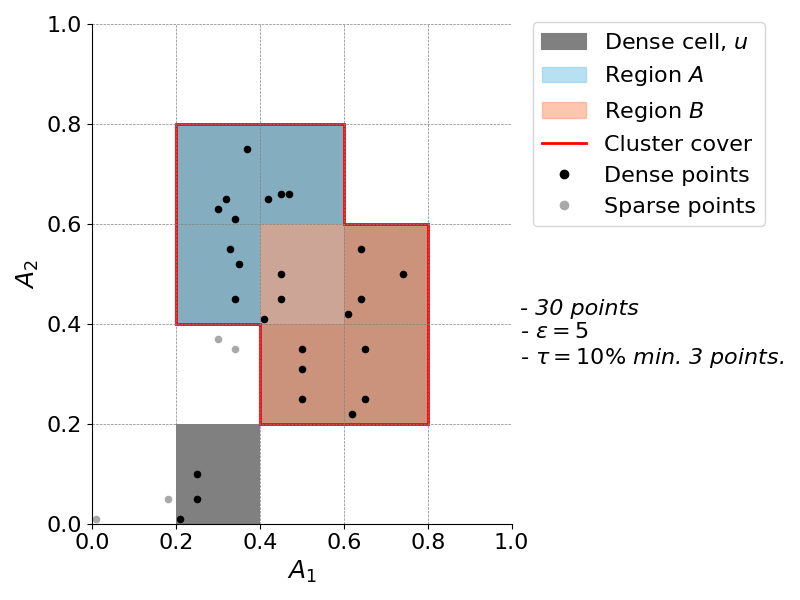
\includegraphics[width=0.35\textwidth]{figures/dense_cells_and_regions.png}
    \caption{Illustration of a dense unit $u$ and two overlapping dense regions $A$ and $B$.}
    \label{fig:dense_cells_and_regions}
    \vspace*{-0.5cm}
\end{figure}

\subsection{Density-based approach}
A big drawback of grid-based methods is that the rely on the grids. In Figure \ref{fig:dense_cells_and_regions} we see that the due to the ragid grid structure we might miss cluster points closely to the dense cells due to non-rectangular cluster shape. Furthermore, This is a limitation of grid-based methods. Density-based methods do not have this limitation, as they do not rely on grids. Instead, they rely on the density of the data points. A well-known density-based clustering algorithm is DBSCAN \cite{dbscan}.


Description of SUBCLU and describe how it relates to DBSCAN.